%----------------------------------------------------------------------------------------
%	PACKAGES AND THEMES
%----------------------------------------------------------------------------------------
\documentclass[aspectratio=169,xcolor=dvipsnames]{beamer}
\usetheme{SimplePlus}
\setbeamercovered{transparent=25}
\AtBeginSection[]
{
    \begin{frame}
        \frametitle{Overview}
        \tableofcontents[currentsection]
    \end{frame}
}

\usepackage{hyperref}
\usepackage{fontenc}
% \hypersetup{colorlinks=true,urlcolor=blue}
% \urlstyle{same}
\usepackage{graphicx} % Allows including images
\usepackage{booktabs} % Allows the use of \toprule, \midrule and \bottomrule in tables
\usepackage{listings,textcomp,color}
\lstset{language=Python,upquote=true,
  basicstyle=\ttfamily\tiny,
  numberstyle=\tiny,stepnumber=1,numbersep=5pt, tabsize=2,
  showspaces=false,showstringspaces=false,showtabs=false,
  breaklines=true,breakatwhitespace=true,escapeinside=||,
  keywordstyle=\color{blue!70},stringstyle=\color{green!70!black!70},
  commentstyle=\color{black!80}\it
}

% ----------------------------------------------------------------------------------------
%	TITLE PAGE
%----------------------------------------------------------------------------------------

\title[short title]{Powerlaw Explained} % The short title appears at the bottom of every slide, the full title is only on the title page
\subtitle{A Guided Tour Through the Mysteries of Force-based Motion Planning}

\author[Day]{Alex Day}

\institute[CU] % Your institution as it will appear on the bottom of every slide, may be shorthand to save space
{
  Ph.D. Student\\
  Motion Planning Lab @ Clemson University\\
  \vspace{5px}
  % Clemson University% Your institution for the title page
}

\date{\today} % Date, can be changed to a custom date


%----------------------------------------------------------------------------------------
%	PRESENTATION SLIDES
%----------------------------------------------------------------------------------------

\begin{document}

\begin{frame}
    % Print the title page as the first slide
    \titlepage
\end{frame}

\begin{frame}{Overview}
    % Throughout your presentation, if you choose to use \section{} and \subsection{} commands, these will automatically be printed on this slide as an overview of your presentation
    \tableofcontents
\end{frame}

%------------------------------------------------
\section{Basics of Motion Planning}
%------------------------------------------------

\begin{frame}{Motion Planning}
    \begin{itemize}
        \item Motion planning is one of the most fundamental skills a human being possesses
        \item Being able to avoid collisions allows us to interact with other humans
        \item Teaching a robot how to approach this problem is very hard
    \end{itemize}
\end{frame}

\begin{frame}{Problem Definition}
    \begin{itemize}
        \item Given a set of agents $A$, each agent has:
        \begin{itemize}
          \item $\mathbf{p}^{t}$ position at time $t$
          \item $\mathbf{v}^{t}$ velocity at time $t$
          \item $\mathbf{g}$ a goal position
          \item $r$ a radius
        \end{itemize}
        \item Each agent is non-holonomic, DOF of the control space equals DOF of the state space
        \item We want:
        \begin{itemize}
          \item $\lvert \mathbf{p}^{-1}_{a} - \mathbf{g}_{a} \rvert < \epsilon$
          \item $\lvert \mathbf{p}^{t}_{a} - \mathbf{p}^{t}_{b} \rvert < r_{a} + r_{b}$
        \end{itemize}
    \end{itemize}
\end{frame}

\begin{frame}{Goal Driving Force}
  \begin{itemize}
    \item Defined as the vector pointing directly at the goal
    \item Getting to the goal is a robots prime directive
  \end{itemize}
  \[
    \mathbf{F}_{goal} = \mathbf{g} - \mathbf{p}
  \]
\end{frame}


\begin{frame}{Current Ecosystem}
  \begin{itemize}
    \item Geometric approaches
    \begin{itemize}
      \item RVO \& ORCA
      \item \textbf{PowerLaw}
      \item Helbing
    \end{itemize}
    \item Learning approaches
    \begin{itemize}
      \item KDMA
      \item CrowdNav/CADRL
      \item NavDreams
    \end{itemize}
  \end{itemize}
\end{frame}

\begin{frame}{Time to Collision}
  \begin{itemize}
    \item Humans use \textit{Time-to-Collision (ttc)}, or $\tau$, as a metric for avoiding collisions
  \end{itemize}
  \begin{figure}
    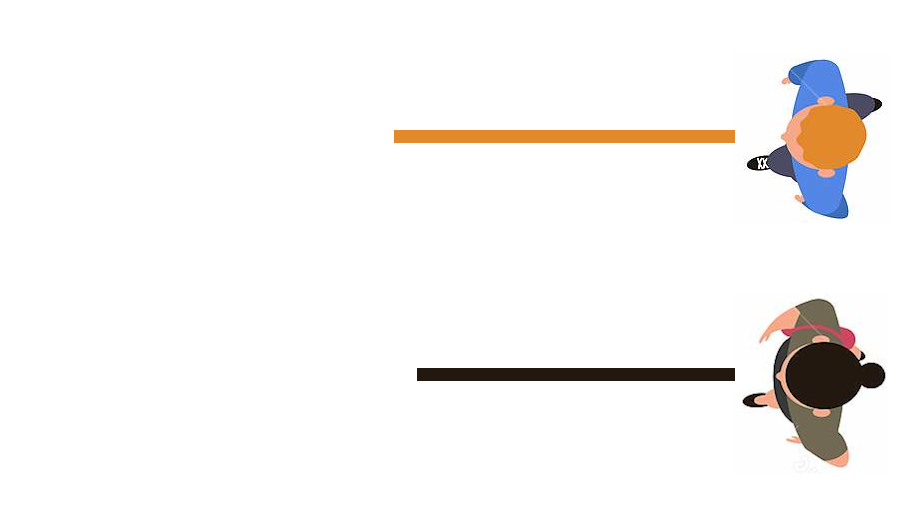
\includegraphics[width=0.7\textwidth]{imgs/no_ttc.png}
  \end{figure}
\end{frame}

\begin{frame}{Time to Collision}
  \begin{itemize}
    \item Humans use \textit{Time-to-Collision (ttc)}, or $\tau$, as a metric for avoiding collisions
  \end{itemize}
  \begin{figure}
    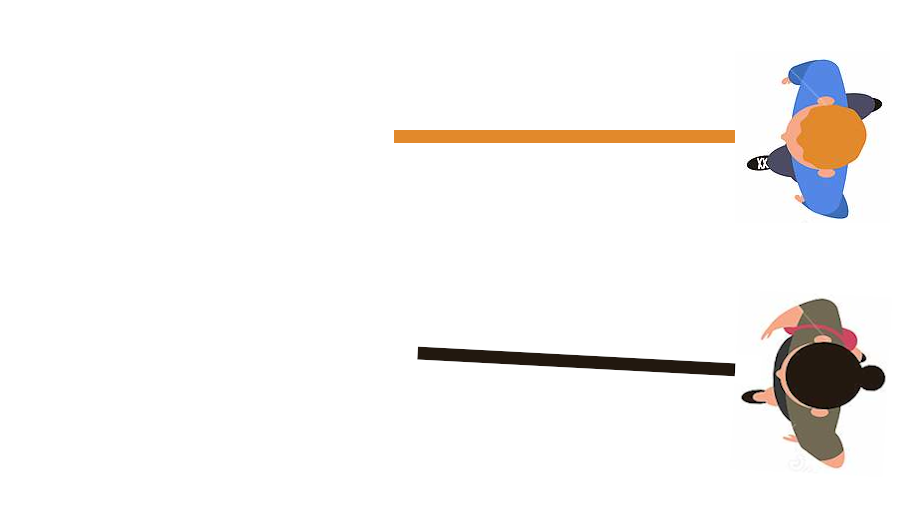
\includegraphics[width=0.7\textwidth]{imgs/ttc_far.png}
  \end{figure}
\end{frame}

\begin{frame}{Time to Collision}
  \begin{itemize}
    \item Humans use \textit{Time-to-Collision (ttc)}, or $\tau$, as a metric for avoiding collisions
  \end{itemize}
  \begin{figure}
    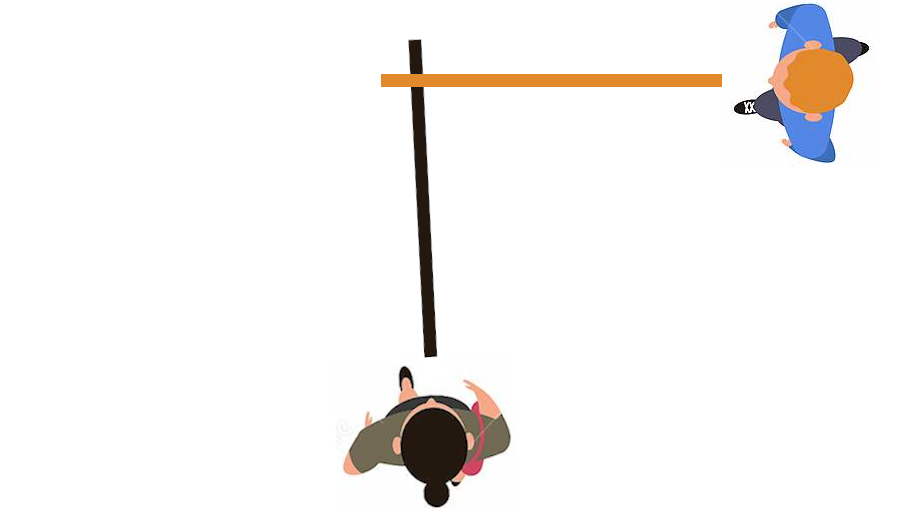
\includegraphics[width=0.7\textwidth]{imgs/ttc_close.png}
  \end{figure}
\end{frame}

\begin{frame}{Powerlaw}
  \begin{itemize}
    \item Humans use \textit{Time-to-Collision (ttc)}, or $\tau$, as a metric for avoiding collisions
    \item When plotting the ttc against a pairwise density function a clear trend emerges
  \end{itemize}
  \begin{figure}
    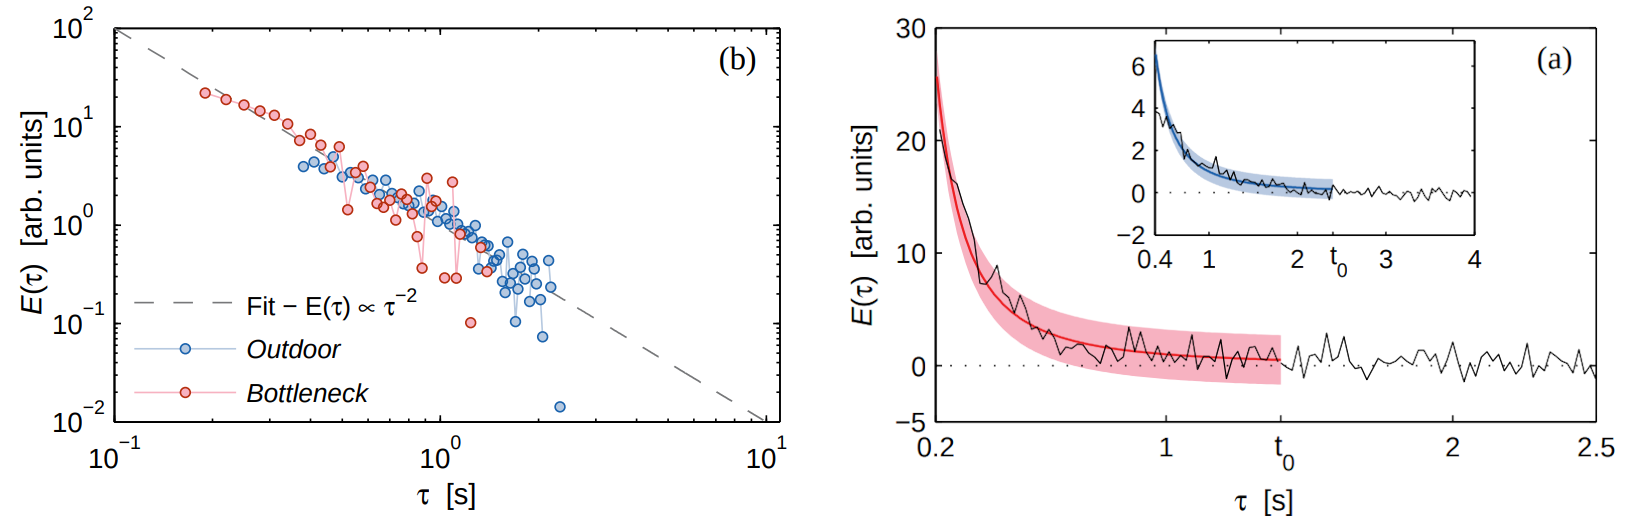
\includegraphics[width=1.0\textwidth]{imgs/pl_graph.png}
  \end{figure}
\end{frame}

\begin{frame}{Powerlaw}
  \begin{itemize}
    \item From that we can generate a model for approximating the energy of a state based on the ttc:
  \end{itemize}
  \begin{gather*}
    E(\tau) = \dfrac{k}{\tau^{2}} e^{-\tau / \tau_{0}}\\\\
    \text{where $\tau$ is the ttc,}\\
    \text{$k$ is a constant that sets the units,}\\
    \text{and $\tau_{0}$ is the time horizon}
  \end{gather*}
\end{frame}

\begin{frame}{Powerlaw}
  \begin{itemize}
    \item This directly implies that the gradient of the energy is the repulsive force experienced by pedestrians
  \end{itemize}
  \begin{gather*}
    \mathbf{F}(\tau) = - \nabla_{\mathbf{r}}\left( \dfrac{k}{\tau^{2}} e^{-\tau / \tau_{0}} \right)\\
    \text{where $\nabla_{\mathbf{r}}$ is the spacial gradient}
  \end{gather*}
  \begin{itemize}
    \item Integrating this force results in a collision free velocity
    \item Combining this with the goal-directed force satisfies both goal-directed behavior and collision-free behavior
  \end{itemize}
\end{frame}

\begin{frame}{High Level}
  \begin{itemize}
    \item There is a force driving each agent to the goal
    \item Each agent enacts some sort of force on every other agent
    \item This inter-agent force is sufficient to avoid all collisions between agents
    \item This combination results in a SOTA decentralized motion planning algorithm
  \end{itemize}
\end{frame}

%------------------------------------------------
\section{Great, now what does that actually mean?}
%------------------------------------------------

\begin{frame}{Context}
\begin{itemize}
  \item Thus far everything has been abstract, so lets contextualize

  \begin{figure}
    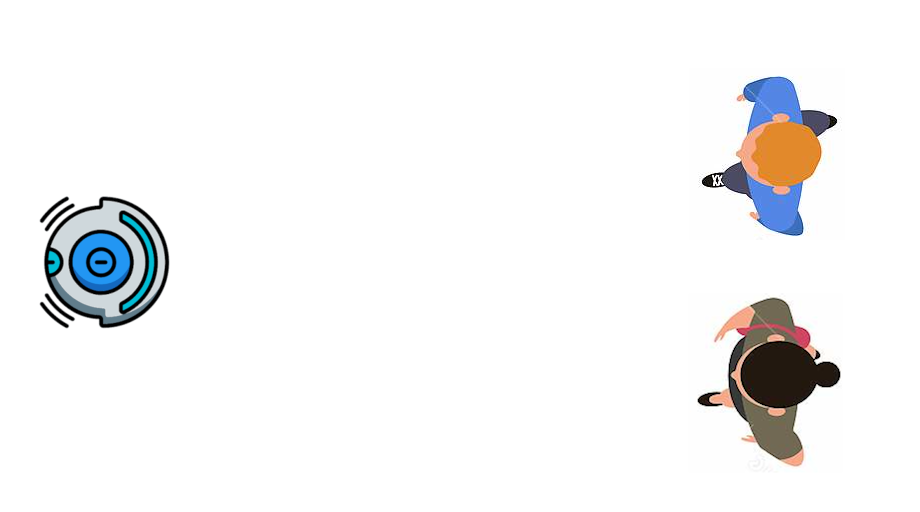
\includegraphics[width=0.6\textwidth]{imgs/scene.png}
  \end{figure}
\end{itemize}
\end{frame}

\begin{frame}{Goal Driving Force}
  \begin{figure}
    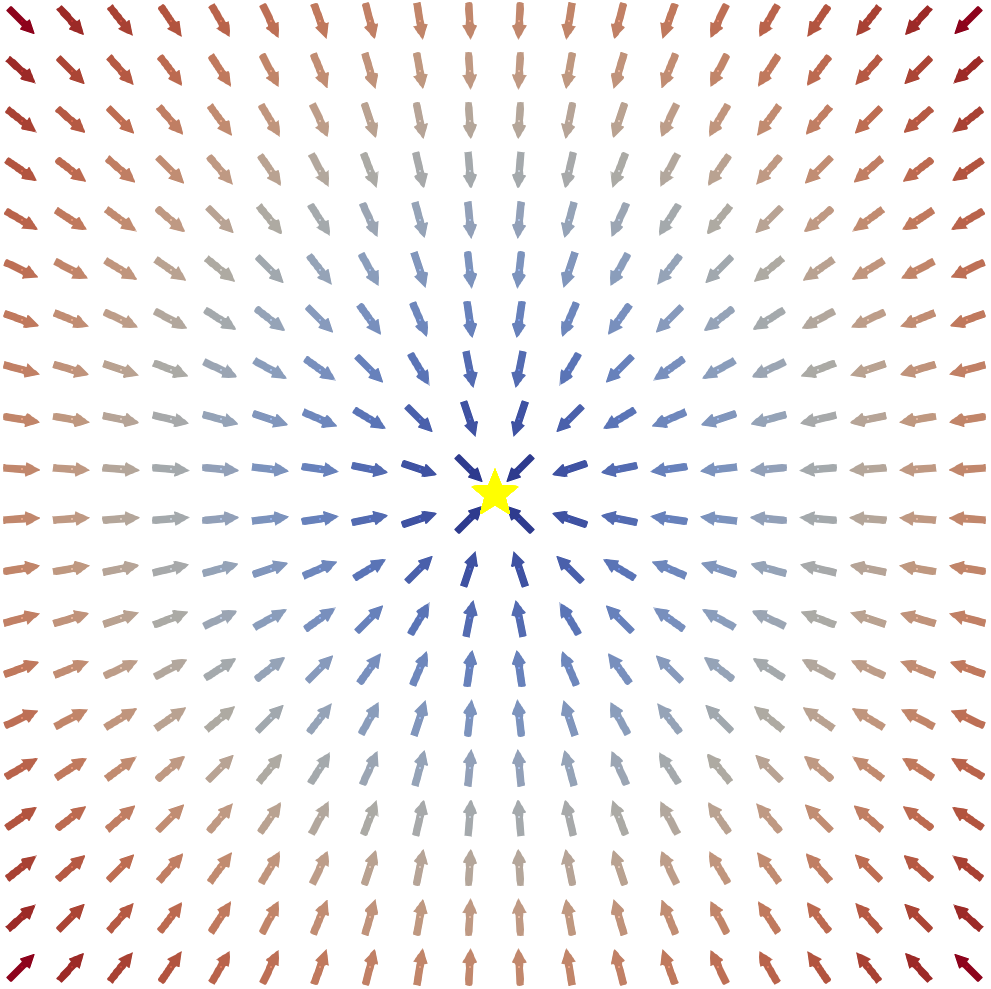
\includegraphics[width=0.5\textwidth]{imgs/goal_directed_force.png}
  \end{figure}
\end{frame}

\begin{frame}{Goal Driving Force}
  \begin{itemize}
    \item Defined as the vector pointing directly at the goal
    \item Getting to the goal is a robots prime directive
  \end{itemize}
  \[
    \mathbf{F}_{goal} = \mathbf{g} - \mathbf{p}
  \]
\end{frame}

\begin{frame}{Goal Driving Force}
  \begin{figure}
    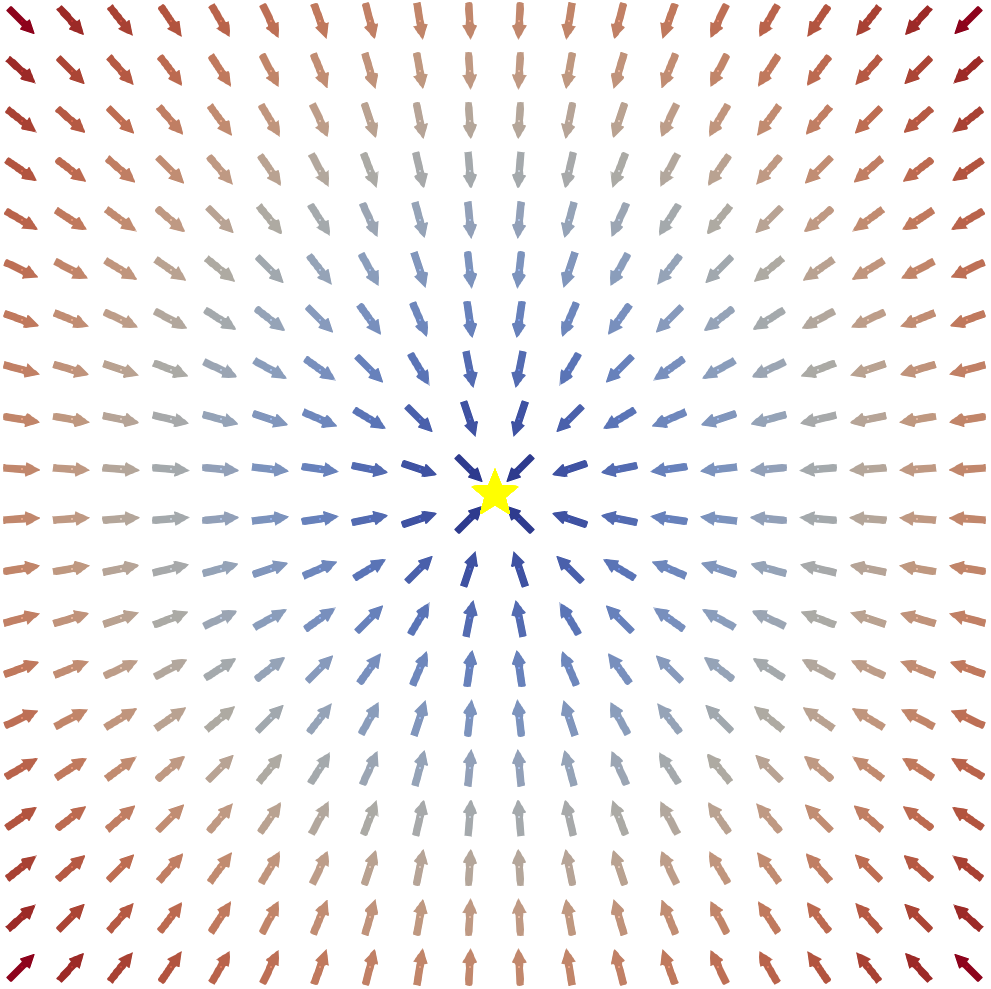
\includegraphics[width=0.5\textwidth]{imgs/goal_directed_force.png}
  \end{figure}
\end{frame}

\begin{frame}{Goal Driving Surface}
  \begin{figure}
    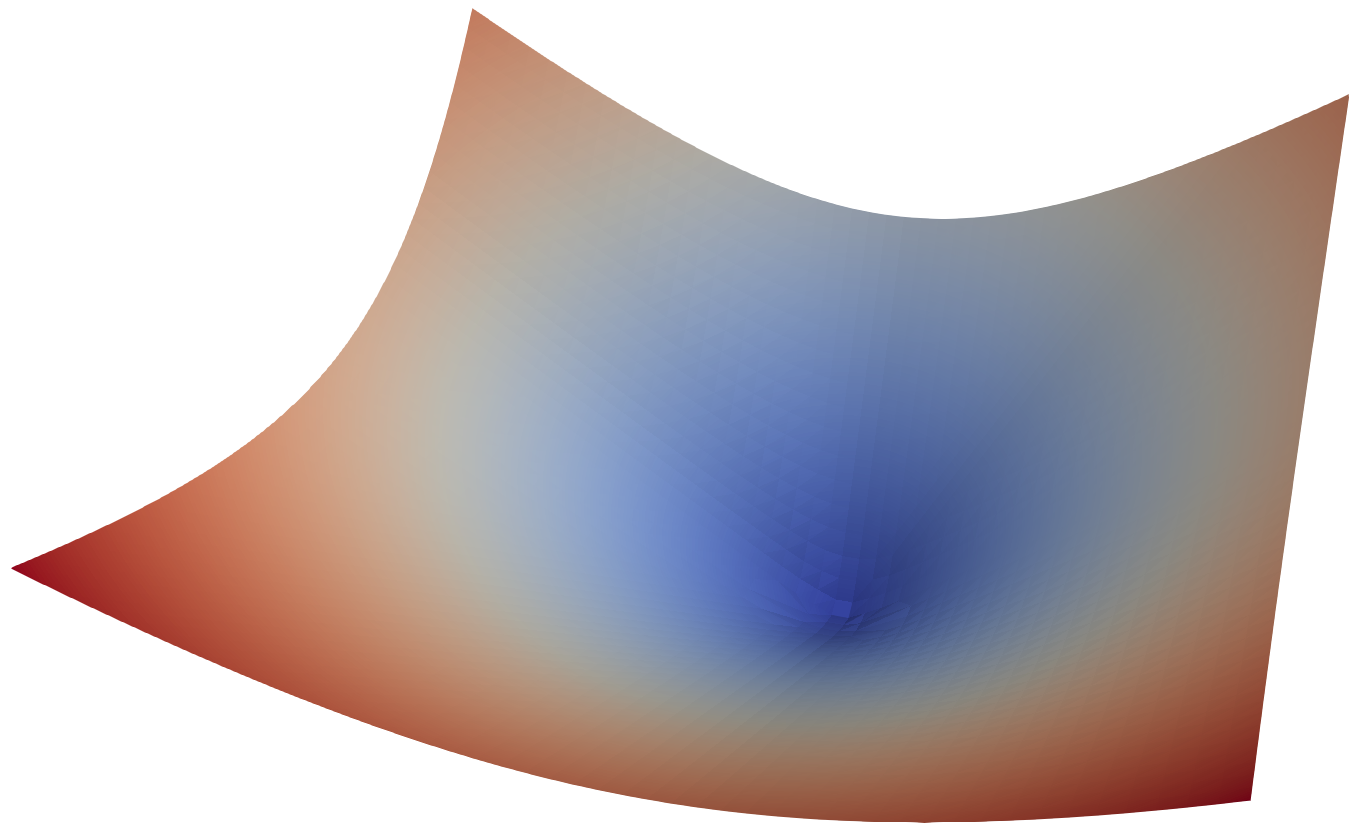
\includegraphics[width=0.5\textwidth]{imgs/goal_surface.png}
  \end{figure}
\end{frame}

\begin{frame}{Combined Induced Forces}
  \begin{figure}
    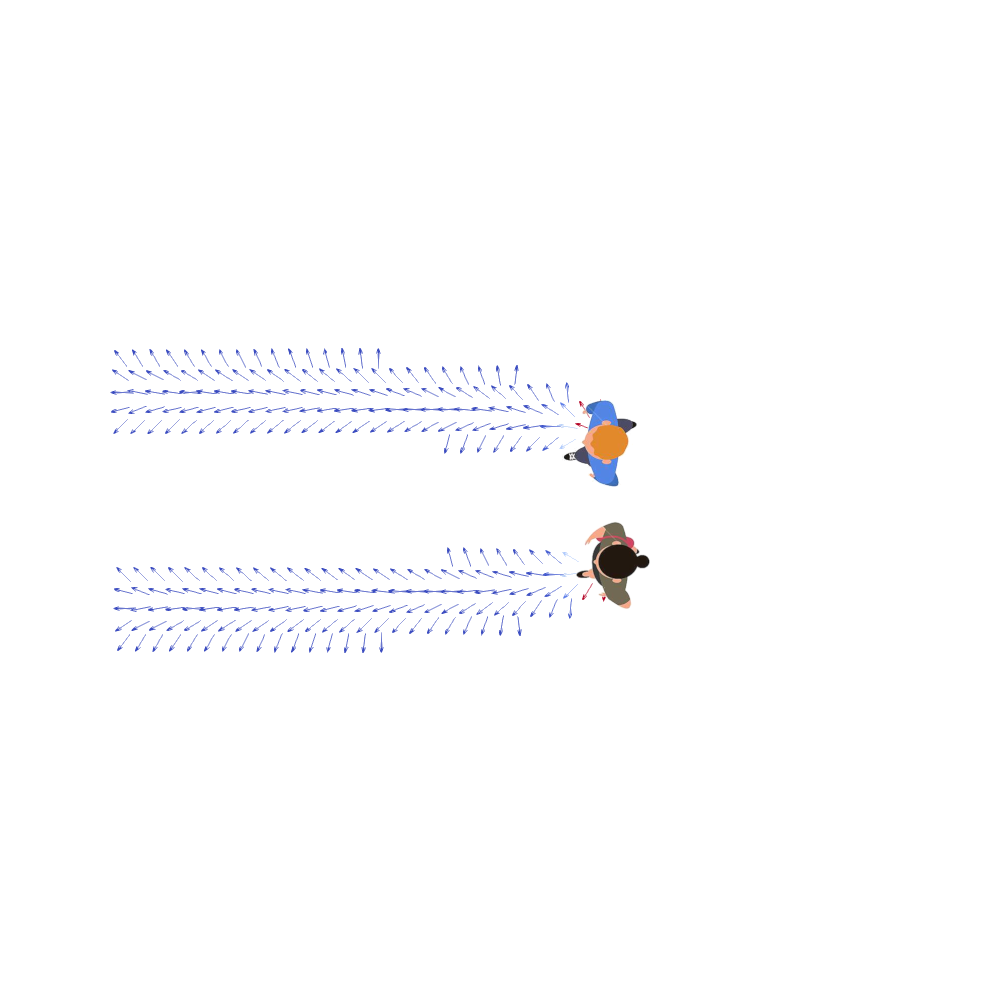
\includegraphics[width=0.5\textwidth]{imgs/combined_forces.png}
  \end{figure}
\end{frame}

\begin{frame}{Combined Induced Forces}
  \begin{figure}
    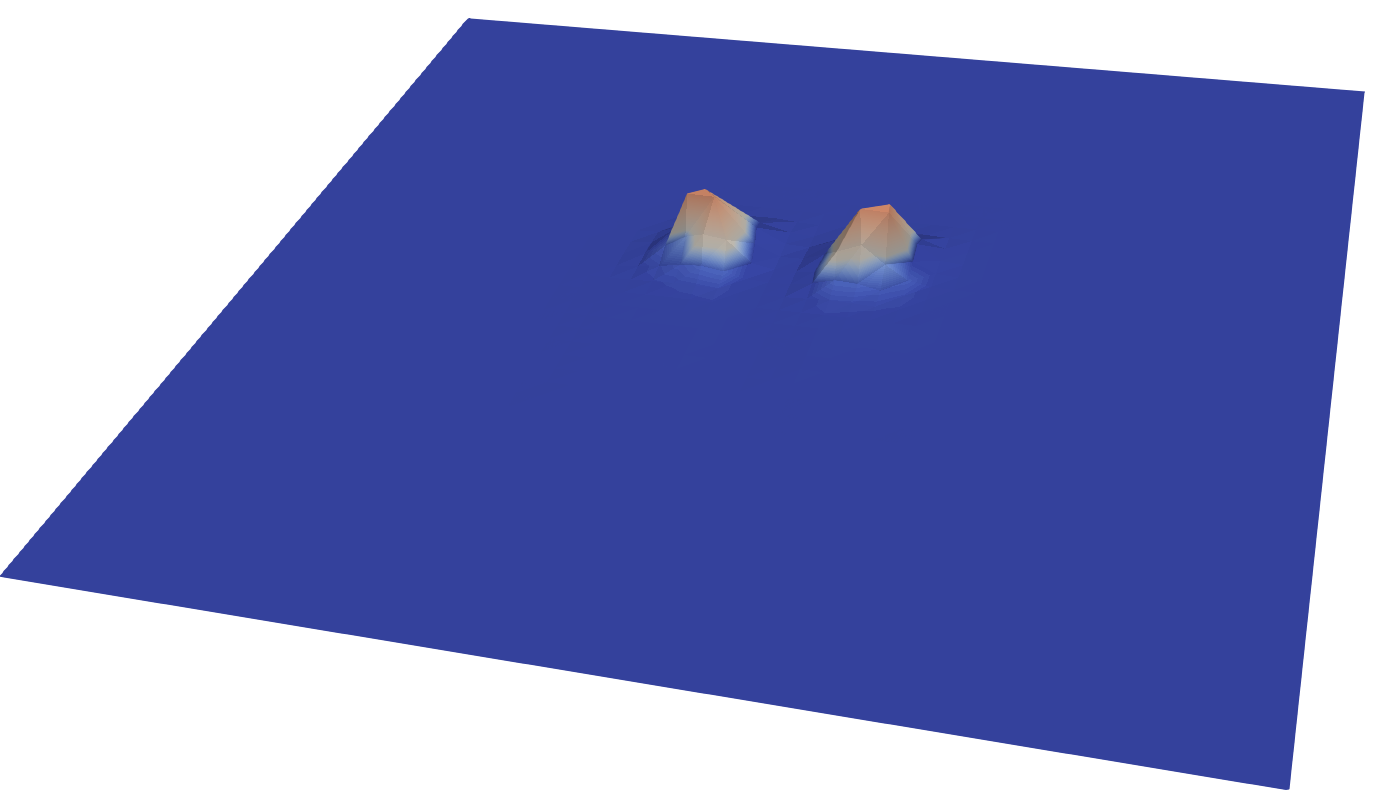
\includegraphics[width=0.5\textwidth]{imgs/forces_surface.png}
  \end{figure}
\end{frame}

\begin{frame}{Powerlaw Forces}
  \begin{figure}
    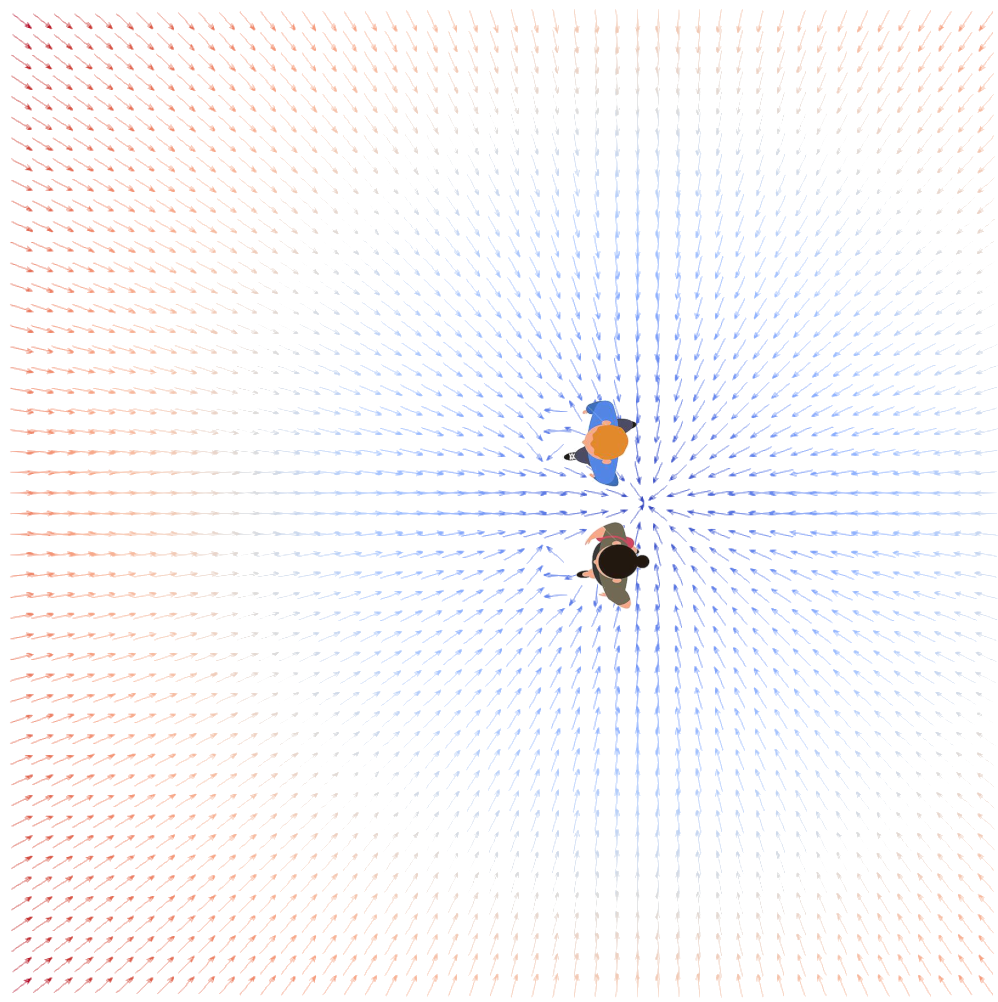
\includegraphics[width=0.5\textwidth]{imgs/final_vel.png}
  \end{figure}
\end{frame}

\begin{frame}{Powerlaw Surface}
  \begin{figure}
    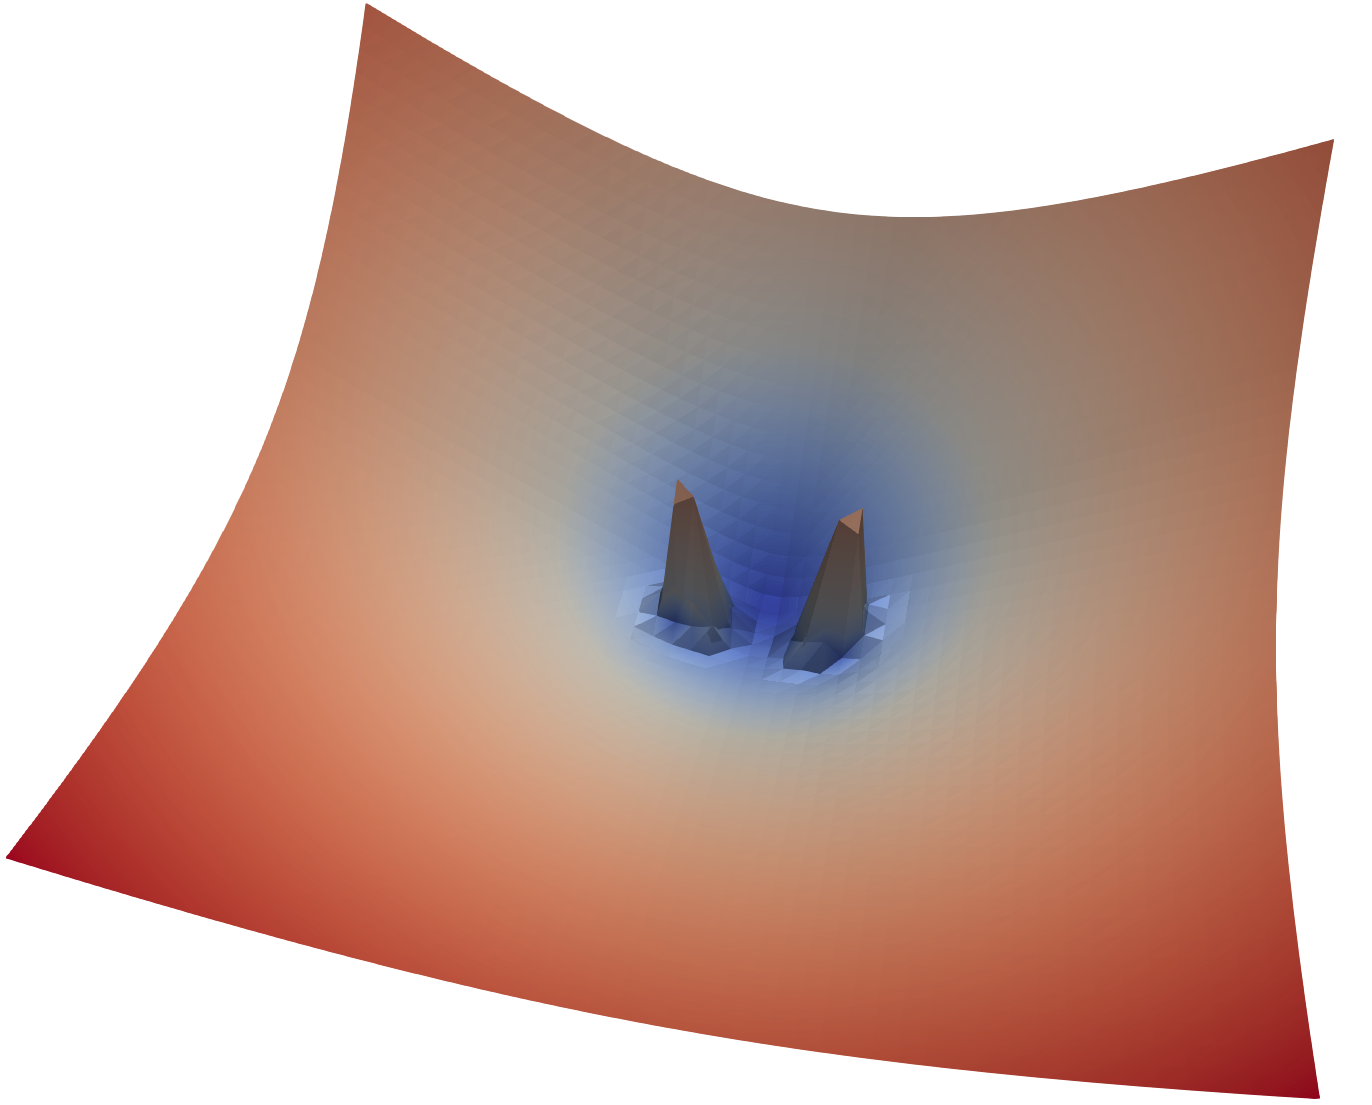
\includegraphics[width=0.5\textwidth]{imgs/final_vel_surface.png}
  \end{figure}
\end{frame}

%------------------------------------------------
\section{Explaining my Visualization Choices}
%------------------------------------------------

\begin{frame}{Simplicity of the Output}
  \begin{itemize}
    \item Motion planning algorithms work mostly with velocities and forces
    \item While there are a decent number of steps in the pipeline, they all deal with something that is relatively basic to visualize
    \item I wanted to build intuition in a similar way to the way a spiral wishing well works
  \end{itemize}
\end{frame}

\begin{frame}{Spiral Wishing Well}
  \begin{figure}
    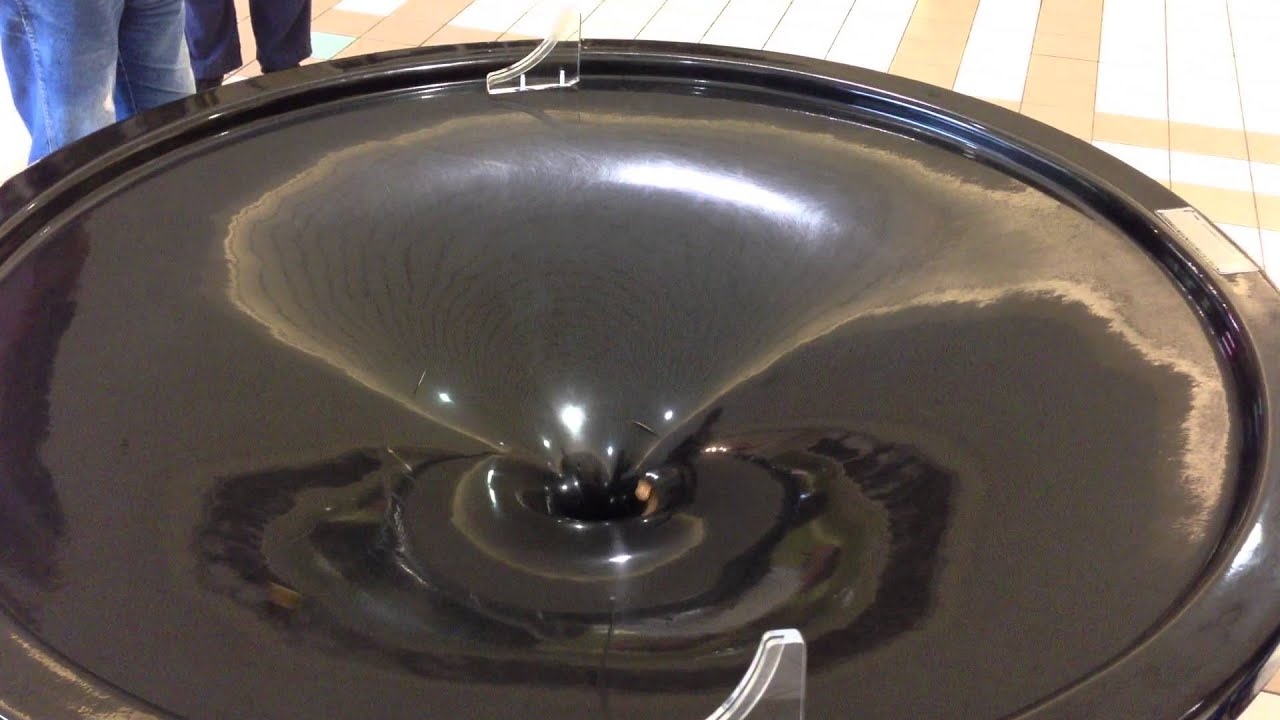
\includegraphics[width=0.75\textwidth]{imgs/spiral_wishing_well.jpg}
  \end{figure}
\end{frame}

\begin{frame}{Vector Fields}
  \begin{itemize}
    \item I couldn't just jump straight to a surface
    \item Vector fields are a good middle ground that show both directionality and magnitude of velocities 
    \item Still have the problem of not really being able to convey how ``strong'' the repulsive force is
  \end{itemize}
\end{frame}

\begin{frame}{Delaunay Triangulation}
  \begin{itemize}
    \item With the Powerlaw algorithm being based on something similar to gradient descent I knew I would have to develop some sort of surface to convey this
    \item Delanunay was a simple way to create that surface
    \item I could vary which of the magnitudes to plot as the z axis, the spacial derivative is something I left to the reader
  \end{itemize}
\end{frame}

%------------------------------------------------
\section{Conclusions and Future Work}
%------------------------------------------------

\begin{frame}{Conclusions}
  \begin{itemize}
    \item Bringing nice visualizations to fruition is both incredibly frustrating and rewarding
    \item A lot of my intuition as to how Powerlaw would look was wrong
    \item As robots become more involved in daily life it will be important to understand how they work
  \end{itemize}
\end{frame}

\begin{frame}{Future Work}
  \begin{itemize}
    \item Visualize in velocity space rather than positional space
    \item Include a ``true" geometric planner like ORCA
    \item Try to visualize something non-numerical, like CrowdNav
  \end{itemize}
\end{frame}

\end{document}
